\logtitle{Example of a quote}{11:21}

\begin{quotation}
    On Ambassador Road, just off I-695 around the corner from the FBI, nearly 100 employees sit in a high-tech suite and wait for terrorists to attack Baltimore. 
    They’ve waited 11 years. But they still have plenty of work to do, like using the intel community’s toys to target this week’s street protests.

  \paragraph{} They are the keepers of the Maryland Coordination and Analysis Center, a government “fusion center” set up to share information and coordinate counterterrorist activities between 29 law enforcement agencies—federal, 
      state, and local, including Baltimore city and county cops—in the aftermath of the Sept. 11 attacks. 
    Seeded by a state anti-terror advisory council whose meetings are closed to the public, nourished by Republican and Democratic governors alike, MCAC has expanded its access to spying tools over the past decade and a half. 
    It can pinpoint cellphone users. It can monitor movements of state motorists through their license plates, as it has done with an estimated 85 million drivers.

  \paragraph{} It turns out that Maryland hasn’t been under sustained assault from international terrorists, despite the wild fears of the homeland security boosters who seek to justify the center’s budget. 
    So rather than accept the possibility that MCAC and other fusion centers were guarding against an overhyped threat, the federal government has expanded the mission to include threats that have always existed: 
    When your job is to find bad guys, it makes it easier to define everyone as a bad guy.

  \paragraph{} The MCAC has adopted what the Department of Homeland Security calls an “all-crimes approach”—one focused not just on monitoring gangs and other criminal threats, but all manners of civil unrest, 
      from Occupy protesters to the Baltimore residents who have clashed with police on the city streets this week. And it is run by a cop who has been accused of racism in the past.

  \sourceatright{\emph{Mike Weinstein, \href{http://phasezero.gawker.com/inside-the-military-police-center-that-spies-on-baltimo-1700670585}{\underline{Phase Zero}}, \formatdate{1}{5}{2015}}}
\end{quotation}

\paragraph{} Nice. Now, for graphics: \\
\noindent%
\begin{minipage}{\linewidth}
\makebox[\linewidth]{
   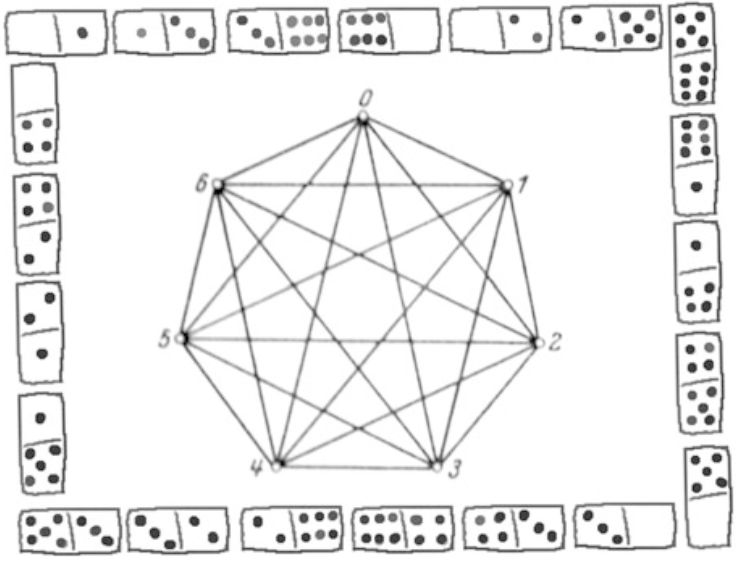
\includegraphics[width=10cm]{2015/6/lol}}
\captionof*{figure}{its a hamiltonian cycle!}
\end{minipage}
Allright.
